%!TEX root = ../thesis.tex

\ifpdf
\graphicspath{{Chapter3/figs/Raster/}{Chapter3/figs/PDF/}{Chapter3/figs/}}
\else
\graphicspath{{Chapter3/figs/Vector/}{Chapter3/figs/}}
\fi

% Create macros to insert tables and tikz figures
\newcommand{\tabpath}[1]{./Chapter3/tables/#1}
\newcommand{\tikzpath}[1]{./Chapter3/figs/#1}
\newcolumntype{b}{X}

% Create new column sizes
\newcolumntype{s}{>{\hsize=.3\hsize}X}
\newcolumntype{t}{>{\hsize=.4\hsize}X}
\newcolumntype{u}{>{\hsize=.5\hsize}X}
\newcolumntype{v}{>{\hsize=.6\hsize}X}

%********************************************************************************
%*********************************** Fourth Chapter *****************************
%********************************************************************************

\chapter{Experimental apparatus and tests procedures}\label{ertp}  

%********************************** First Section  *******************************
\section[Experimental assembly]{Experimental assembly}\label{ertp:expt}

  Lorem ipsum dolor sit amet, consectetur adipiscing elit. Sed vel congue lorem, nec aliquam ex. Nulla quis dui vel eros volutpat viverra a vitae odio. Maecenas non venenatis augue. Mauris eros est, lacinia sit amet rhoncus vel, molestie et dolor. Donec sapien lectus, dignissim a tellus mattis, dignissim varius lectus. In venenatis nibh turpis, sit amet porttitor elit dictum non. In in dictum leo. Suspendisse vestibulum nunc augue, ac bibendum risus hendrerit ac. In dui turpis, ultrices vitae pulvinar ac, maximus nec justo. Morbi tincidunt, nunc sit amet facilisis luctus, nunc sem lobortis erat, sit amet ornare orci tortor ut ex. Curabitur ut lacus dui.

  Donec ipsum sem, ultrices et tristique eget, fringilla in enim. Ut id varius tellus, sit amet rhoncus nulla. Fusce lacinia enim eget mi elementum fringilla. Nulla facilisi. Aenean vitae urna porta ipsum tempor lacinia quis id ligula. Nam lobortis neque nec arcu convallis laoreet. Orci varius natoque penatibus et magnis dis parturient montes, nascetur ridiculus mus. Pellentesque habitant morbi tristique Table \ref{tab:lline_cmp} senectus et netus et malesuada fames ac turpis egestas. 

  \input{\tabpath{lline_cmp.tex}}
  
  Integer eget tempor velit. Duis rhoncus ligula id nunc rutrum gravida. Phasellus at imperdiet neque. Praesent fringilla a nibh ac egestas. Mauris vel porttitor elit, quis faucibus erat. Ut viverra justo id nisl gravida, quis tristique leo venenatis. Donec magna neque, maximus vel convallis eu, consequat lobortis orci. Pellentesque placerat enim vitae arcu malesuada, nec convallis eros dapibus. Aenean vitae mi volutpat, mattis lorem sit amet, ultricies magna. Integer convallis congue quam, eget maximus turpis blandit eget. Nullam lorem quam, condimentum quis eleifend eget, ultricies ac eros. Sed porttitor molestie ante a scelerisque. Aliquam erat volutpat. Duis arcu elit, laoreet consequat sapien eget, suscipit scelerisque magna. Praesent leo justo, Figure \ref{fig:fem} scelerisque eget rutrum id, faucibus in dui. 

  \begin{figure}[!htb]
    \centering
    \input{\tikzpath{fem_tikz.tex}}
    \caption[FEM]{FEM with notes in the photo.}
    \label{fig:fem}
  \end{figure}

%********************************** %Sixth Section  **************************************
\section[Experimental procedure]{Experimental procedure}\label{ertp:exp_proc}
  
  Integer eget tempor velit. Duis rhoncus ligula id nunc rutrum gravida. Phasellus at imperdiet neque. Praesent fringilla a nibh ac egestas. Mauris vel porttitor elit, quis faucibus erat. Ut viverra justo id nisl gravida, quis tristique leo venenatis. Donec magna neque, maximus vel convallis eu, consequat lobortis orci. Pellentesque placerat enim vitae arcu malesuada, nec convallis eros dapibus. Aenean vitae mi volutpat, mattis lorem sit amet, ultricies magna.
  
  \begin{figure}[!htb]
    \centering
    \input{\tikzpath{exp_proc.tex}}
    \caption[Experimental procedure flowchart.]{Experimental procedure flowchart.}
    \label{fig:fchart_exp}
  \end{figure}
  

%********************************** %Seventh Section  ************************************
\section[Test matrix]{Test matrix}\label{ertp:mtx}
  
  Integer convallis congue quam, eget maximus turpis blandit eget. Nullam lorem quam, condimentum quis eleifend eget, ultricies ac eros. Sed porttitor molestie ante a scelerisque. Aliquam erat volutpat. Duis arcu elit, laoreet consequat sapien eget, suscipit scelerisque magna. Praesent leo justo, scelerisque eget rutrum id, faucibus in dui. Maecenas a dolor id elit condimentum mattis nec id turpis.

  Nullam non justo cursus sapien porttitor malesuada vitae et diam. Ut sed imperdiet dolor, sed volutpat metus. Nam at est condimentum, consectetur tortor quis, accumsan lorem. Mauris vel ex eu purus pellentesque dictum. Morbi vulputate mollis elit. Vestibulum auctor diam eu ligula interdum finibus. In hac habitasse platea dictumst. Cras non ultricies metus. Aliquam eget nibh eget ex accumsan sagittis nec ac mauris. Suspendisse consectetur tellus quis purus porttitor, ac tincidunt urna dictum. In dictum neque quis lorem ullamcorper condimentum \ref{fig:tst_mtx}.

  \begin{figure}[!htb]
      \centering
      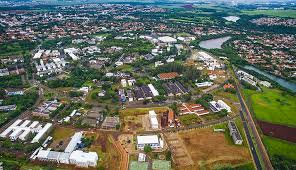
\includegraphics[width=0.75\textwidth, keepaspectratio]{unicamp.jpg}
      \caption[Test matrix.]{ Test matrix as function of the liquid and gas superficial velocities.}
      \label{fig:tst_mtx}
  \end{figure}

  Donec interdum lacus neque, a scelerisque nisl pharetra at. Curabitur a iaculis odio. Interdum et malesuada fames ac ante ipsum primis in faucibus. Pellentesque habitant morbi tristique senectus et netus et malesuada fames ac turpis egestas. Sed vulputate augue a urna ullamcorper egestas. Maecenas ligula lectus, porta non facilisis eget, finibus vel nisi. Ut finibus sollicitudin nisl, ut lacinia enim consequat sed.

  \begin{figure}[!htb]
    \begin{subfigure}{0.48\textwidth}
      \includegraphics[width=\linewidth, height=0.6\textheight, keepaspectratio=True]{./sub/cepetro.jpg}
      \caption{CEPETRO.} 
      \label{fig:CEPETRO}
    \end{subfigure}
    \hspace*{\fill} % separation between the subfigures
    \begin{subfigure}{0.48\textwidth}
      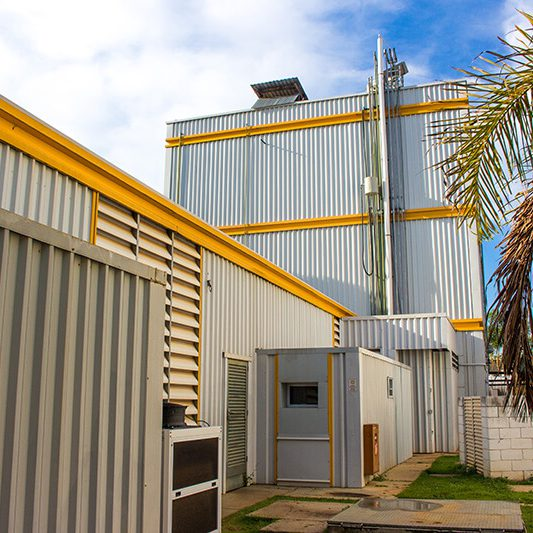
\includegraphics[width=\linewidth, height=0.6\textheight, keepaspectratio=True]{./sub/labpetro.jpg}
      \caption{LABPETRO.}
      \label{fig:LABPETRO}
    \end{subfigure}
  \end{figure}
